\documentclass[11pt,a4paper]{article}

\usepackage[utf8]{inputenc}
\usepackage[margin=0.85in]{geometry}
\usepackage{amsmath,amssymb}
\usepackage{booktabs}
\usepackage{tabularx}
\usepackage{graphicx}
\usepackage{hyperref}
\usepackage{enumitem}
\usepackage{listings}
\usepackage{xcolor}

\hypersetup{
    colorlinks=true,
    linkcolor=blue!75!black,
    urlcolor=blue!75!black,
    citecolor=blue!75!black
}

\setlist[itemize]{noitemsep, topsep=2pt}
\setlist[enumerate]{noitemsep, topsep=2pt}

\lstset{
    basicstyle=\ttfamily\footnotesize,
    breaklines=true,
    frame=single,
    backgroundcolor=\color{gray!8},
    rulecolor=\color{gray!30},
    keywordstyle=\color{blue!80!black}\bfseries,
    commentstyle=\color{green!50!black}\itshape,
    stringstyle=\color{red!60!black},
    numbers=none
}

\title{\textbf{ESP32 Classical Key Exchange Benchmark}\\[0.2em]\large Phase A: Isolated Micro-Benchmarks (No Network Involved)\\[0.2em]\normalsize FYP Documentation: Embedded VPN Client (Deliverable 3)}
\author{Department of Computer Engineering}
\date{October 2026}

\begin{document}

\maketitle

\section{Phase A: Isolated Micro-Benchmarks (No Network Involved)}

Phase A benchmarks the raw cryptographic execution of three key exchange schemes on an ESP32-D0WDQ6 microcontroller running at 240~MHz. Tests run locally in chip memory without network stack overhead to profile pure computational cost, memory allocation, and payload footprint:
\begin{enumerate}
    \item \textbf{X25519:} Modern Montgomery-curve Diffie-Hellman algorithm over Curve25519 (RFC~7748).
    \item \textbf{ECDH P-256:} Standard NIST elliptic curve algorithm over secp256r1.
    \item \textbf{Classical DH-2048:} Classic Finite Field Diffie-Hellman configured with RFC~3526 2048-bit MODP prime.
\end{enumerate}

\section{Key Performance Indicators (KPIs)}

The evaluation profiles six Key Performance Indicators (KPIs) covering execution latency, hardware workload, wire footprint, and RAM consumption.

\subsection{KPI Definitions and Operational Impact}

\begin{itemize}
    \item \textbf{KEX-1 (Key Generation Time):} Elapsed time to generate a fresh ephemeral public and private key pair. Determines the latency overhead when creating ephemeral keys for session forward secrecy.
    \item \textbf{KEX-2 (Public Key Size):} Encoded byte length of the public key transmitted over the network channel.
    \item \textbf{KEX-3 (Secret Derivation Time):} Elapsed time to compute the shared secret from the peer's public key.
    \item \textbf{KEX-4 (Shared Secret Size):} Encoded byte length of the derived shared secret output fed into HKDF for symmetric session key derivation.
    \item \textbf{KEX-5 (Total Client Compute Time):} Total on-chip processor time ($\text{KEX-1} + \text{KEX-3}$) required for complete client key exchange.
    \item \textbf{KEX-6 (Peak Dynamic Heap Memory):} Dynamic RAM allocated from the ESP32 heap during cryptographic operations. Excessive allocations risk Out-Of-Memory (OOM) resets.
    \item \textbf{Hardware CPU Cycles (@ 240 MHz):} Hardware processor cycles consumed during execution. Because the ESP32 clock operates at 240~MHz (240,000,000 cycles per second), hardware cycle counts provide an exact, clock-invariant metric:
    \begin{equation}
    \text{Time (ms)} = \frac{\text{CPU Cycles}}{240,000}
    \end{equation}
\end{itemize}

\subsection{Iteration Count Strategy}

\begin{itemize}
    \item \textbf{Benchmark Iterations ($N = 100$):} All three algorithms (X25519, ECDH P-256, and DH-2048) were executed 100 times to compute stable arithmetic means and cancel out OS scheduling jitter.
    \item \textbf{FreeRTOS Watchdog Mitigation:} In Classical DH-2048, periodic yields (\texttt{vTaskDelay(1)}) prevent Task Watchdog Timer (TWDT) resets during heavy modular exponentiation loops.
\end{itemize}

\begin{table}[htbp]
\centering
\small
\caption{Summary of Key Exchange Benchmarking KPIs}
\label{tab:kex_kpis}
\begin{tabularx}{\textwidth}{lll X}
\toprule
\textbf{KPI ID} & \textbf{Metric Name} & \textbf{Unit} & \textbf{Operational Significance for Embedded VPN} \\
\midrule
\textbf{KEX-1} & Key Generation Time & ms / cycles & Time spent generating client ephemeral keypair \\
\textbf{KEX-2} & Public Key Wire Size & Bytes & Network transmission payload per session \\
\textbf{KEX-3} & Secret Derivation Time & ms / cycles & Time spent computing shared secret from peer key \\
\textbf{KEX-4} & Shared Secret Output Size & Bytes & Output size fed into HKDF key derivation \\
\textbf{KEX-5} & Total Client Compute Time & ms / cycles & Total CPU time ($\text{KEX-1} + \text{KEX-3}$) per handshake \\
\textbf{KEX-6} & Peak Dynamic Heap RAM & Bytes & Dynamic RAM consumed during test \\
\bottomrule
\end{tabularx}
\end{table}

\section{Comparison Tables}

\subsection{Performance Comparison}

Table~\ref{tab:comparison_summary} summarizes the empirical metrics collected across all three algorithms on the ESP32 at 240~MHz, indicating the best performer for each parameter.

\begin{table}[htbp]
\centering
\small
\setlength{\tabcolsep}{3.2pt}
\caption{Performance Comparison: X25519 vs. ECDH P-256 vs. Classical DH-2048}
\label{tab:comparison_summary}
\begin{tabular}{l c c c c c}
\toprule
\textbf{Metric} & \textbf{X25519} & \textbf{ECDH P-256} & \textbf{DH-2048} & \textbf{Winner} & \textbf{Performance Factor} \\
\midrule
\multicolumn{6}{l}{\textbf{Execution Latency (Milliseconds)}} \\
Key Generation Time     & \textbf{8.47 ms}   & 156.83 ms & 31.60 ms & \textbf{X25519} & $18.5\times$ faster than P-256 \\
Secret Derivation Time  & \textbf{16.91 ms}  & 156.73 ms & 31.44 ms & \textbf{X25519} & $9.3\times$ faster than P-256 \\
Total Client Crypto Time& \textbf{25.38 ms}  & 313.56 ms & 63.04 ms & \textbf{X25519} & $12.4\times$ faster than P-256 \\
\midrule
\multicolumn{6}{l}{\textbf{Hardware CPU Cycles (@ 240 MHz)}} \\
KeyGen Cycles           & \textbf{2,033,095} & 37,638,242 & 7,583,754 & \textbf{X25519} & Lowest compute workload \\
Derivation Cycles       & \textbf{4,057,917} & 37,615,903 & 7,546,518 & \textbf{X25519} & Lowest compute workload \\
Total Client Cycles     & \textbf{6,091,012} & 75,254,145 & 15,130,272 & \textbf{X25519} & Lowest compute workload \\
\midrule
\multicolumn{6}{l}{\textbf{Communication Payload (Bytes)}} \\
Public Key Size         & \textbf{32 bytes}  & 65 bytes   & 256 bytes & \textbf{X25519} & $8.0\times$ smaller than DH-2048 \\
Shared Secret Size      & 32 bytes           & 32 bytes   & 256 bytes & ---             & 256-bit symmetric key seed \\
Total Data Footprint    & \textbf{64 bytes}  & 97 bytes   & 512 bytes & \textbf{X25519} & $8.0\times$ smaller than DH-2048 \\
\midrule
\multicolumn{6}{l}{\textbf{Memory Utilization}} \\
Peak Dynamic Heap RAM   & \textbf{0 bytes}   & 348 bytes  & 636 bytes & \textbf{X25519} & Stack only (0 bytes heap) \\
\bottomrule
\end{tabular}
\end{table}

\section{Selection Rationale for X25519}

X25519 was selected as the key exchange scheme for the ESP32 VPN client based on four critical technical advantages:

\begin{enumerate}
    \item \textbf{Minimal Computation Latency (2.5x to 12.4x speed advantage):} X25519 completes key generation in \textbf{8.47~ms} and secret derivation in \textbf{16.91~ms}, totaling \textbf{25.38~ms}. In comparison, Classical DH-2048 requires \textbf{63.04~ms} ($2.48\times$ slower) and ECDH P-256 requires \textbf{313.56~ms} ($12.35\times$ slower). The entire X25519 key exchange executes in approximately 25~ms, eliminating connection setup bottlenecks.
    
    \item \textbf{Compact Wire Payload (8x smaller than DH-2048):} X25519 requires only \textbf{32 bytes} on the wire for the public key, compared to 65 bytes for ECDH P-256 (uncompressed format) and 256 bytes for DH-2048. The compact 32-byte payload fits into single-packet envelopes, avoids MTU fragmentation, and minimizes Wi-Fi radio transmission time to preserve battery life.
    
    \item \textbf{Zero Heap Memory Overhead (0 bytes vs. 348 and 636 bytes):} The ESP32 has approximately 320~KB of usable RAM shared among Wi-Fi drivers, network buffers, and RTOS queues. X25519 consumes \textbf{0 bytes of dynamic heap memory}, executing purely within the local stack frame. In contrast, ECDH P-256 allocates 348 bytes and DH-2048 allocates 636 bytes for multi-precision integer contexts, introducing memory fragmentation risks.
    
    \item \textbf{Deterministic Constant-Time Timing \& Side-Channel Resistance:} X25519 utilizes the Montgomery ladder algorithm, which naturally executes in constant time regardless of the private key value, preventing timing and power side-channel attacks. Furthermore, any 32-byte array constitutes a valid Curve25519 point, eliminating point-on-curve validation checks that are prone to implementation bugs in Weierstrass curves like P-256.
    
    \item \textbf{Rationale for Hardcoded RFC 3526 MODP Prime in DH-2048:} In Classical DH-2048, safe prime generation ($p = 2q + 1$) dynamically at runtime on an ESP32 is computationally prohibitive, requiring minutes of Miller-Rabin primality testing and causing watchdog timeouts. The standardized RFC~3526 2048-bit MODP prime is mathematically verified, provides instant initialization, and prevents small-subgroup confinement attacks.
\end{enumerate}

\section{Serial Monitor Output Verification}

The terminal captures below confirm execution runs and heap measurements recorded on the ESP32 hardware:

\subsection{Detailed Per-Algorithm Execution Capture}

Figure~\ref{fig:term_detailed} displays the serial output across 100 runs, showing exact cycle counts, converted millisecond timings, wire sizes, and peak dynamic heap RAM for X25519, ECDH P-256, and DH-2048.

\begin{figure}[htbp]
\centering
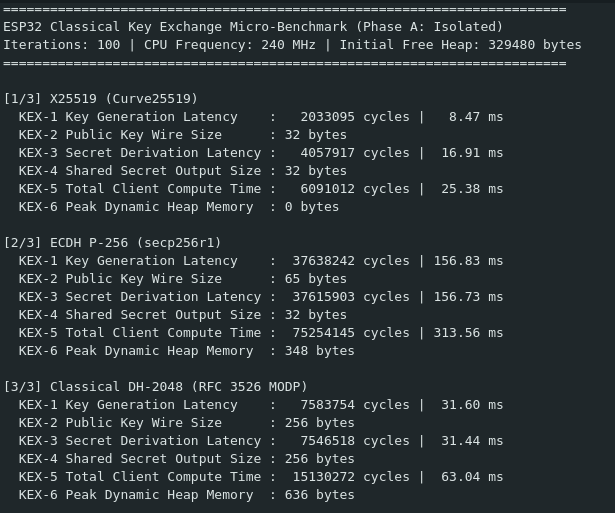
\includegraphics[width=0.85\textwidth]{screenshots/terminal_detailed_runs.png}
\caption{ESP32 Serial Output for Key Exchange Micro-Benchmarks (100 runs, 240 MHz).}
\label{fig:term_detailed}
\end{figure}

\subsection{Benchmark Results Summary Table Capture}

Figure~\ref{fig:term_summary} displays the terminal output summarizing all tested algorithms across all evaluated KPIs (KEX-1 through KEX-6).

\begin{figure}[htbp]
\centering
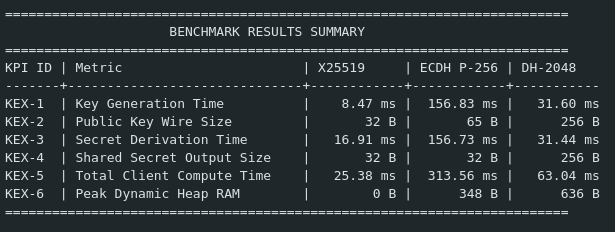
\includegraphics[width=0.85\textwidth]{screenshots/terminal_summary_table.png}
\caption{ESP32 Serial Output showing the automated Benchmark Results Summary Table.}
\label{fig:term_summary}
\end{figure}

\section{Graphical Benchmark Visualizations}

The figures below plot the empirical metrics across execution latency, communication payload, and heap memory:

\subsection{Execution Latency Comparison}

Figure~\ref{fig:plot_timing} compares key generation, secret derivation, and total compute latency on a logarithmic scale.

\begin{figure}[htbp]
\centering
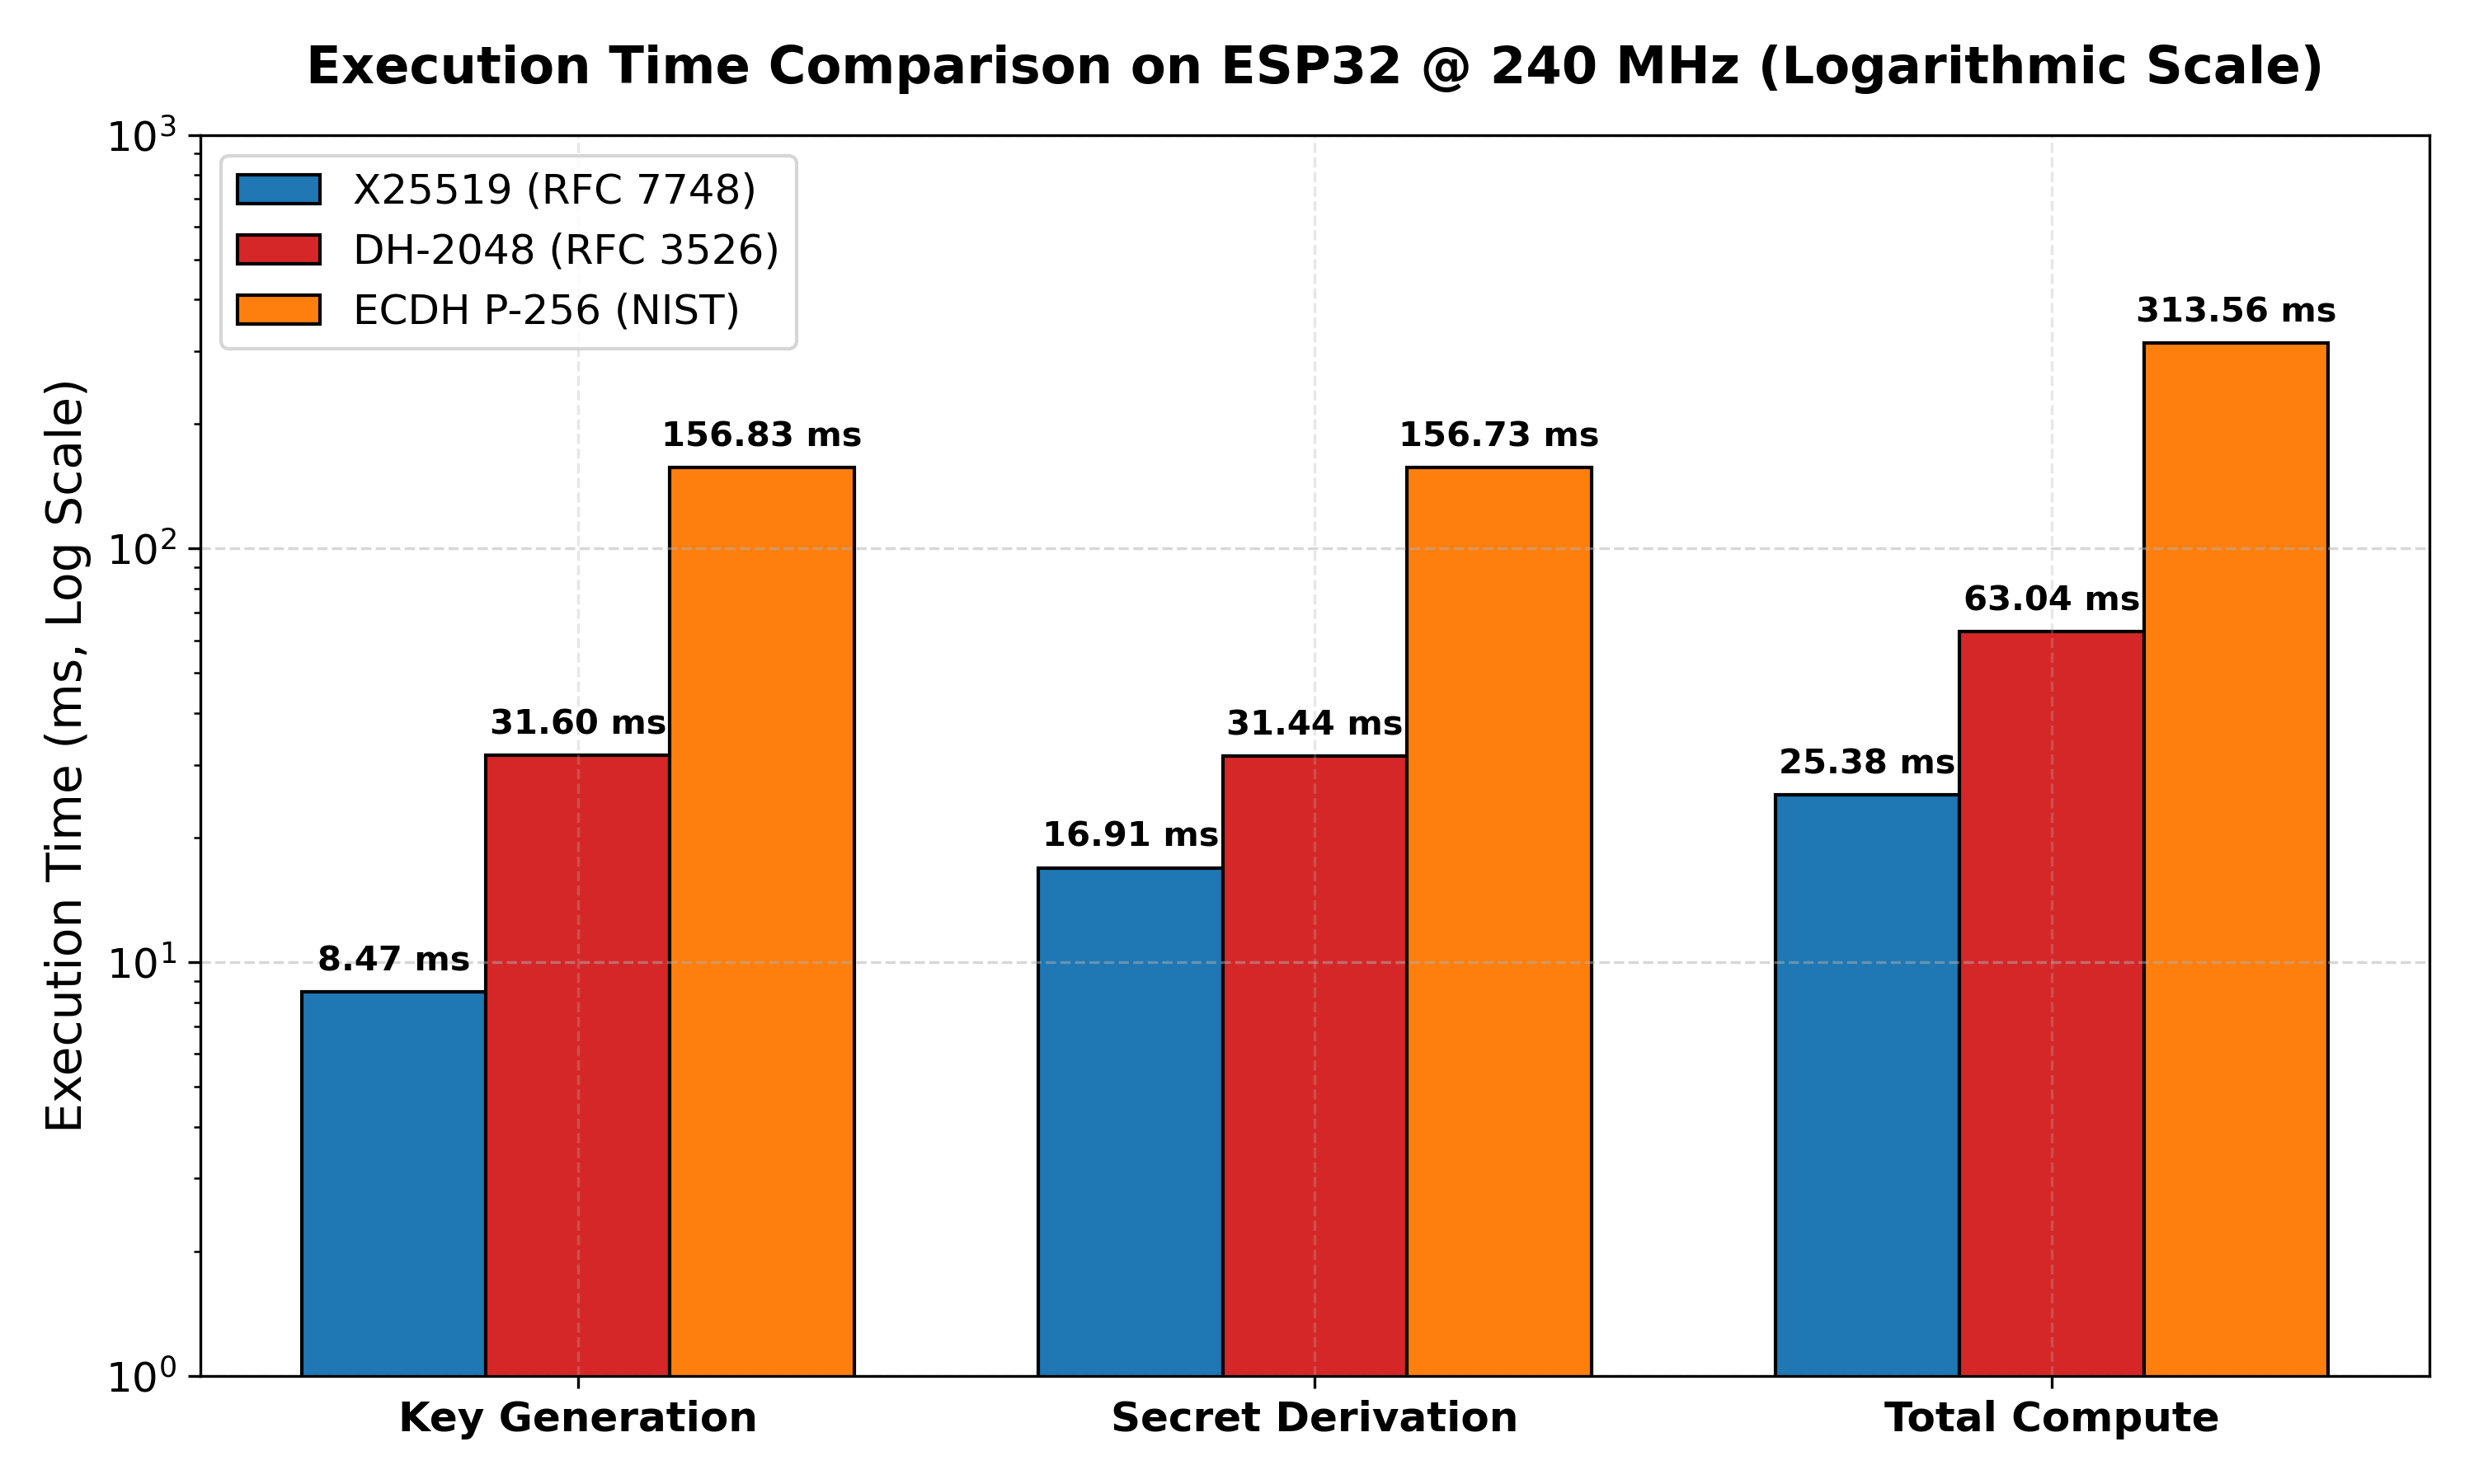
\includegraphics[width=0.80\textwidth]{graphs/fig_timing_comparison.png}
\caption{Execution time comparison (logarithmic scale) for KeyGen, Secret Derivation, and Total Compute.}
\label{fig:plot_timing}
\end{figure}

\subsection{Handshake Communication Overhead}

Figure~\ref{fig:plot_wire} breaks down public key and shared secret output sizes in bytes.

\begin{figure}[htbp]
\centering
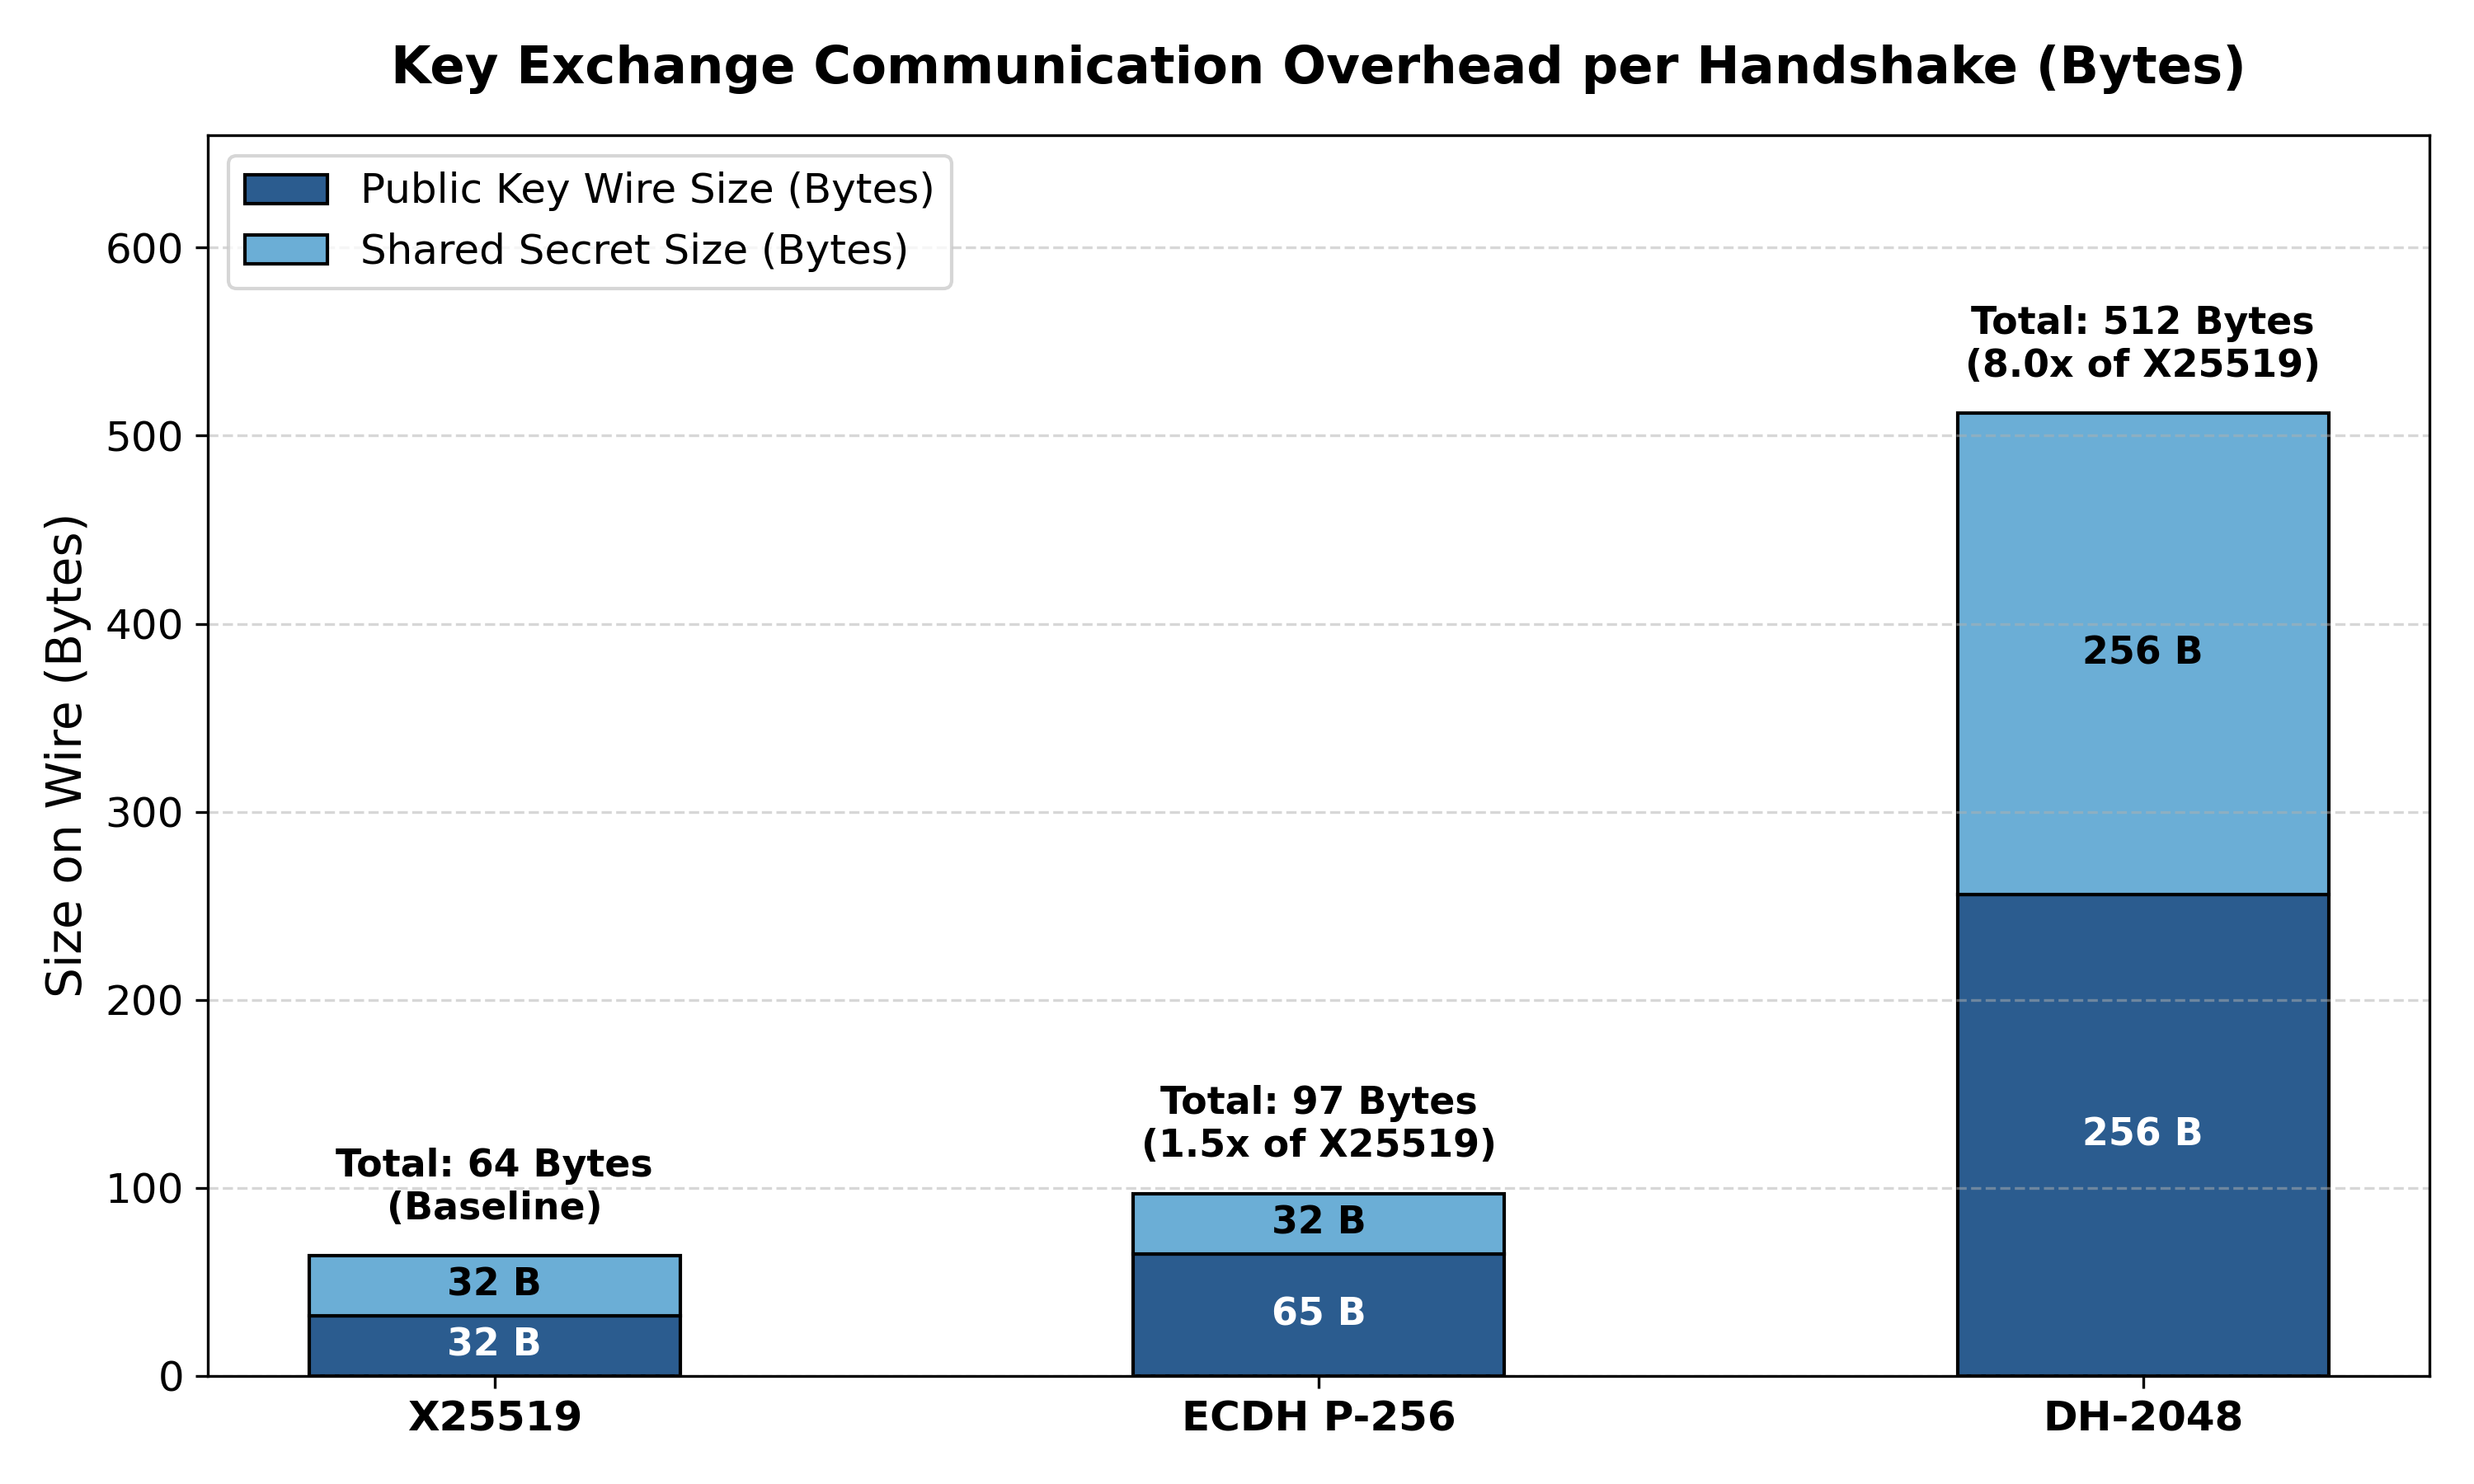
\includegraphics[width=0.80\textwidth]{graphs/fig_size_overhead.png}
\caption{Key exchange communication overhead (Public Key + Shared Secret size in bytes).}
\label{fig:plot_wire}
\end{figure}

\subsection{Dynamic Heap Memory Overhead}

Figure~\ref{fig:plot_memory} illustrates the peak dynamic heap RAM consumed during algorithm execution.

\begin{figure}[htbp]
\centering
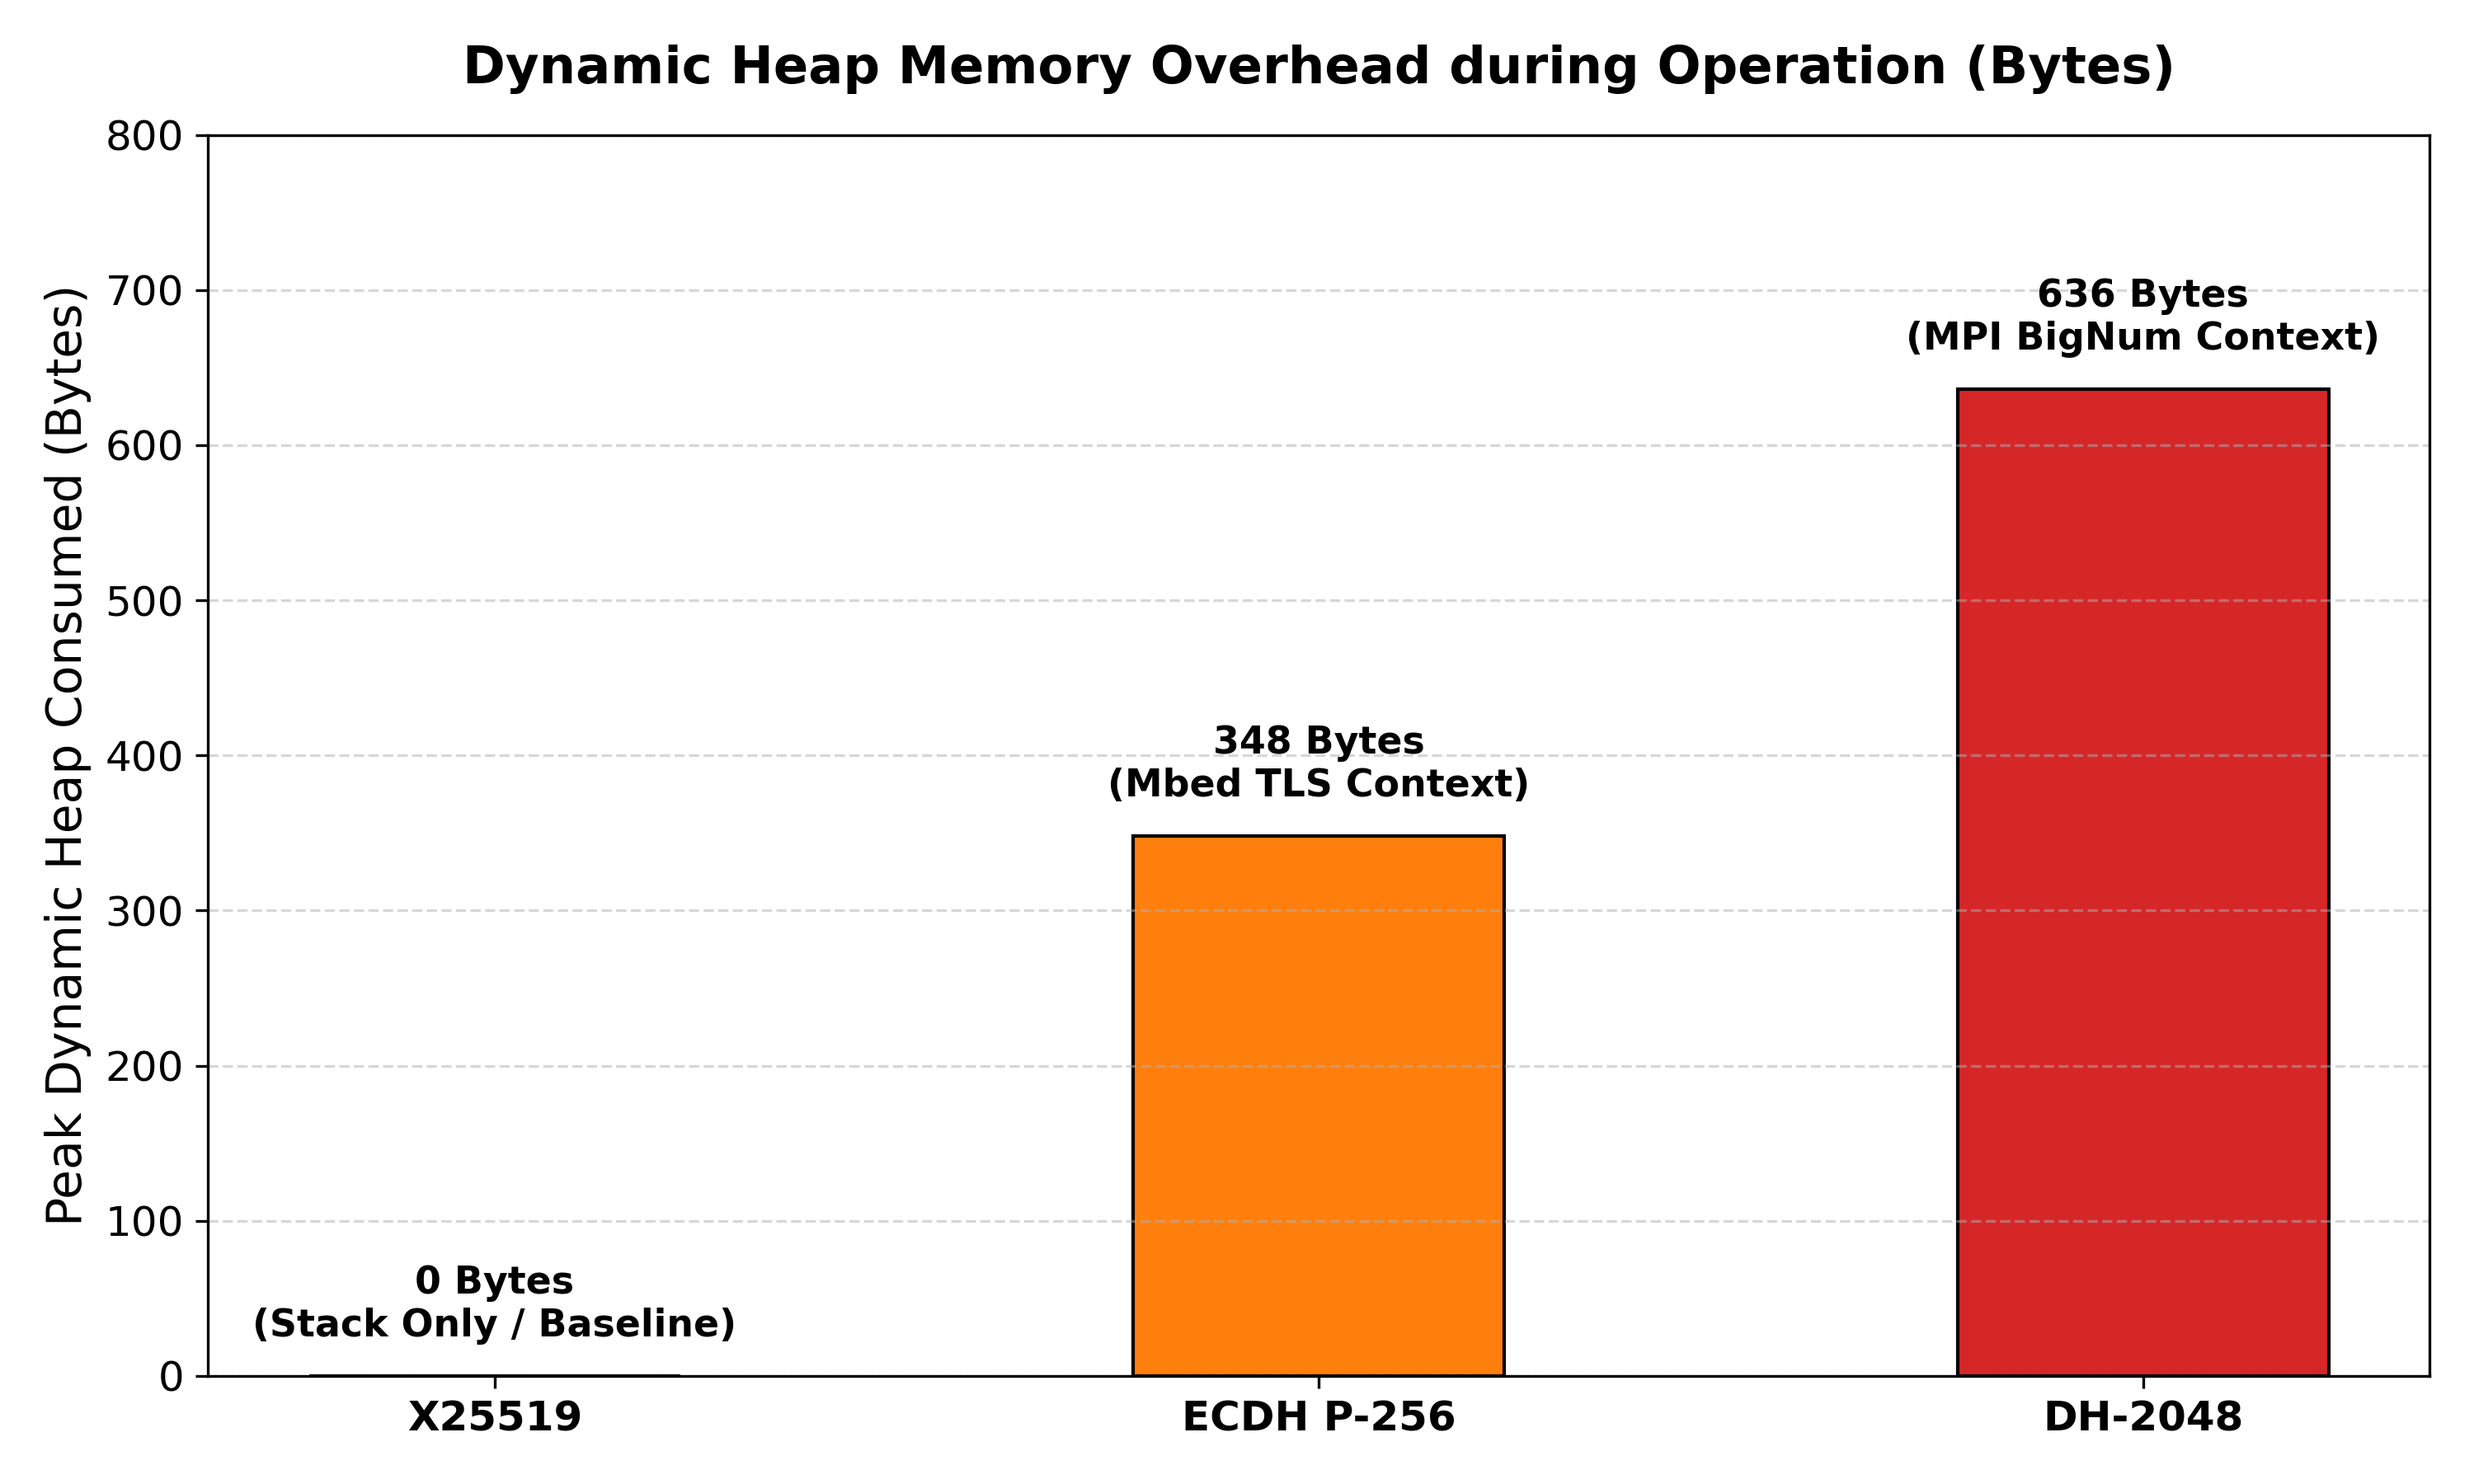
\includegraphics[width=0.80\textwidth]{graphs/fig_memory_comparison.png}
\caption{Dynamic heap memory consumed by each key exchange algorithm on the ESP32.}
\label{fig:plot_memory}
\end{figure}

\section{Benchmarking Logic and Pseudocode}

The pseudocode below details the measurement routine implemented on the ESP32, including cycle counter acquisition, heap profiling, and test loops for each algorithm:

\subsection{Setup and Hardware Measurement Helpers}

\begin{lstlisting}[language=C++]
// Configuration: ESP32 runs at 240 MHz clock speed
const uint32_t CPU_FREQ_MHZ = 240;
const int ITERATIONS = 100;

// Reads 32-bit hardware cycle register directly from ESP32 core
static inline uint32_t read_cpu_cycles() {
  uint32_t ccount;
  __asm__ __volatile__("rsr %0, ccount" : "=a"(ccount));
  return ccount;
}

// Converts raw CPU clock cycles into milliseconds
float cycles_to_ms(uint32_t cycles) {
  return (float)cycles / (CPU_FREQ_MHZ * 1000.0f);
}
\end{lstlisting}

\subsection{X25519 Benchmark Routine}

\begin{lstlisting}[language=C++]
// Target KPIs: KEX-1 (KeyGen), KEX-2 (Wire: 32 B), KEX-3 (Deriv), KEX-4 (Secret: 32 B), KEX-5 (Total Compute), KEX-6 (Heap)
uint8_t client_pk[32], client_sk[32], peer_pk[32], peer_sk[32], shared[32];
crypto_kx_keypair(peer_pk, peer_sk);

uint32_t heap_before = ESP.getFreeHeap();
uint32_t peak_heap = 0;

for (int i = 0; i < ITERATIONS; i++) {
  // [KEX-1] Ephemeral Key Generation & [KEX-2] Public Key Size (32 bytes)
  uint32_t t0 = read_cpu_cycles();
  crypto_kx_keypair(client_pk, client_sk);
  uint32_t t1 = read_cpu_cycles();
  time_keygen[i] = t1 - t0;

  // [KEX-6] Peak Dynamic Heap RAM Profiling (Stack execution: 0 bytes)
  uint32_t used_heap = heap_before - ESP.getFreeHeap();
  if (used_heap > peak_heap) peak_heap = used_heap;

  // [KEX-3] Shared Secret Derivation & [KEX-4] Shared Secret Output Size (32 bytes)
  uint32_t t2 = read_cpu_cycles();
  crypto_scalarmult(shared, client_sk, peer_pk);
  uint32_t t3 = read_cpu_cycles();
  time_derive[i] = t3 - t2;

  // [KEX-5] Total Client Compute Cycles = KEX-1 + KEX-3
}
\end{lstlisting}

\subsection{ECDH P-256 Benchmark Routine}

\begin{lstlisting}[language=C++]
// Target KPIs: KEX-1 (KeyGen), KEX-2 (Wire: 65 B), KEX-3 (Deriv), KEX-4 (Secret: 32 B), KEX-5 (Total Compute), KEX-6 (Heap: 348 B)
mbedtls_ecp_group grp;
mbedtls_mpi peer_d, client_d, shared_z;
mbedtls_ecp_point peer_Q, client_Q;
// ... initialize contexts and RNG ...
mbedtls_ecp_group_load(&grp, MBEDTLS_ECP_DP_SECP256R1);
mbedtls_ecdh_gen_public(&grp, &peer_d, &peer_Q, mbedtls_ctr_drbg_random, &random_gen);

uint32_t heap_before = ESP.getFreeHeap();
uint32_t peak_heap = 0;

for (int i = 0; i < ITERATIONS; i++) {
  // [KEX-1] Ephemeral Keypair Generation & [KEX-2] Public Key Wire Size (65 bytes uncompressed)
  uint32_t t0 = read_cpu_cycles();
  mbedtls_ecdh_gen_public(&grp, &client_d, &client_Q, mbedtls_ctr_drbg_random, &random_gen);
  uint32_t t1 = read_cpu_cycles();
  time_keygen[i] = t1 - t0;

  // [KEX-6] Peak Dynamic Heap RAM Profiling (Captures Mbed TLS context allocation: 348 B)
  uint32_t used_heap = heap_before - ESP.getFreeHeap();
  if (used_heap > peak_heap) peak_heap = used_heap;

  // [KEX-3] Shared Secret Derivation & [KEX-4] Shared Secret Output Size (32 bytes)
  uint32_t t2 = read_cpu_cycles();
  mbedtls_ecdh_compute_shared(&grp, &shared_z, &peer_Q, &client_d, mbedtls_ctr_drbg_random, &random_gen);
  uint32_t t3 = read_cpu_cycles();
  time_derive[i] = t3 - t2;

  // [KEX-5] Total Client Compute Cycles = KEX-1 + KEX-3
}
\end{lstlisting}

\subsection{Classical DH-2048 Benchmark Routine}

\begin{lstlisting}[language=C++]
// Target KPIs: KEX-1 (KeyGen), KEX-2 (Wire: 256 B), KEX-3 (Deriv), KEX-4 (Secret: 256 B), KEX-5 (Total Compute), KEX-6 (Heap: 636 B)
mbedtls_mpi P, G, peer_X, peer_Y, client_X, client_Y, shared_K;
// ... initialize MPI contexts and load RFC 3526 2048-bit MODP prime and generator G=2 ...

uint32_t heap_before = ESP.getFreeHeap();
uint32_t peak_heap = 0;

for (int i = 0; i < ITERATIONS; i++) {
  // [KEX-1] Key Generation: Random Exponent client_X & Modular Exponentiation client_Y = G^X mod P
  // [KEX-2] Public Key Wire Size (256 bytes)
  uint32_t t0 = read_cpu_cycles();
  mbedtls_mpi_fill_random(&client_X, 32, mbedtls_ctr_drbg_random, &random_gen);
  mbedtls_mpi_exp_mod(&client_Y, &G, &client_X, &P, NULL);
  uint32_t t1 = read_cpu_cycles();
  time_keygen[i] = t1 - t0;

  // [KEX-6] Peak Dynamic Heap RAM Profiling (Captures BigNum MPI context allocations: 636 B)
  uint32_t used_heap = heap_before - ESP.getFreeHeap();
  if (used_heap > peak_heap) peak_heap = used_heap;

  // [KEX-3] Shared Secret Derivation: shared_K = peer_Y^client_X mod P
  // [KEX-4] Shared Secret Output Size (256 bytes)
  uint32_t t2 = read_cpu_cycles();
  mbedtls_mpi_exp_mod(&shared_K, &peer_Y, &client_X, &P, NULL);
  uint32_t t3 = read_cpu_cycles();
  time_derive[i] = t3 - t2;

  // [KEX-5] Total Client Compute Cycles = KEX-1 + KEX-3
  if (i % 10 == 0) vTaskDelay(1); // FreeRTOS watchdog mitigation
}
\end{lstlisting}

\end{document}
